%------------------------------------------------------------------------------%
% bachelor thesis															   %
% create by: Mario Preishuber												   %
% create date: 2014, Jan 01.												   %
%------------------------------------------------------------------------------%

\documentclass[10pt,fleqn, titlepage]{article}
\usepackage{oldgerm}
\usepackage{graphicx}
\usepackage{xspace}
\usepackage[numbers]{natbib}
\usepackage{url}
\usepackage{subcaption}
\usepackage{booktabs}

%Macro definitions
\newcommand{\JS}{JavaScript\xspace}
\newcommand{\SM}{SpiderMonkey\xspace}
\newcommand{\ACDCJS}{ACDC4JS\xspace}


\graphicspath{
	{../imgs/}
	{../imgs/plots/}
	{../imgs/plots/mutator/}
	{../imgs/plots/system/}
	{../imgs/plots/system_vs_mutator/}
}

\textheight     230mm
\textwidth      165mm
\topmargin      -10mm
\oddsidemargin    0mm
\evensidemargin   0mm

\makeatletter
\def\input@path{{./extras/}{./chapters/}}
\makeatother

\begin{document}
	
	%\maketitle
	
	\begin{titlepage}
		\centering

		\vspace*{\fill}
		{\LARGE 
		Bachelor Thesis									\\ \bigskip
		\textbf{Observation of Real-World Web Applications 
		to Obtain an Realistic \JS Heap Behavior}}		\\ \bigskip
		~ \\ \bigskip
		\Large Mario Preishuber 						\\ \smallskip
		\large
		\texttt{mario.preishuber@cs.uni-salzburg.at}	\\ \bigskip
		Department of Computer Sciences					\\ \smallskip			
		University of Salzburg							\\ \smallskip
		Austria											\\ \bigskip 
		~ \\ \bigskip
		\today
		\vspace*{\fill}
		
		\textbf{Advisor} 								\\ \bigskip
		Professor Christoph Kirsch						\\ \smallskip
		\texttt{ck@cs.uni-salzburg.at}					\\ \bigskip
	\end{titlepage}
	
	\bibliographystyle{unsrtnat}
	
	% add tables of content
	%-------------------------------------------------------------------
% bachelor thesis
%
% topic: ACDC4JS - How to analyze a JavaScript garbage collector
%
% create by: Mario Preishuber
% create date: 2014, Jan 01.
%-------------------------------------------------------------------

\tableofcontents
\listoffigures
\listoftables
	
	% add abstract
	%------------------------------------------------------------------------------%
% bachelor thesis															   %
% create by: Mario Preishuber												   %
% create date: 2014, Jan 01.												   %
%------------------------------------------------------------------------------%
\begin{abstract}

\begin{table}[h]
\centering
\begin{tabular}{c}
\parbox{0.7\linewidth}{


    \JS performance is a hot topic for pushing the boundaries of web
    applications.  Today, browser vendors compare to each other mainly on \JS
    benchmark scores rather than other web browsing features. However, recent
    studies~\cite{JSMeter2009} suggest that popular benchmarking suites do not
    reflect the behavior of real web applications.  We present an extensive
    analysis of \JS heaps in 11 real-world web applications to aid the
    development of more realistic workloads for benchmarking the memory
    management of \JS virtual machines. In this thesis, we confirm empirical
    results on object type and object lifetime distribution~\cite{JSMeter2009}
    and contribute new insights on object size distribution as well as heap
    structure properties. TODO: eventuall kannst du hier noch einen Satz anbringen
    der die Ergebnisse beschreibt. Aber nicht mehr als ein Satz. Sowas wie:
    Our results suggest that \JS applications typically allocate mostly
    small and short living objects and that blablabla is more likely than bla.

%Improving the performance of a \JS virtual machines is a hot topic. There are
%industry-standard benchmark suites to support implementation and optimization
%of \JS virtual machines, but studies, like \cite{JSMeter2009}, illustrate that
%these benchmarks do not represent a real-world web application behavior. Since
%\JS is a garbage collected programming language improving performance of the
%memory management of a \JS virtual machine may improve performance in general.
%To be able to improve performance it requires better understanding performance
%deficiencies. To optimize a \JS virtual machine a configurable and realistic
%benchmarking of memory management is needed. Realistic benchmarking is only
%possible if typical \JS heaps are known. This requires intensive analysis of
%\JS heaps of real-world applications.

%We propose our analysis results of \JS heaps of real-world applications. Our
%analysis results support developer to implement realistic benchmarking suites
%which are able to simulate realistic \JS heap behavior. We study 11 popular
%real-world web applications. Depending on the analyzed application we executed
%different user interactions. We use a sampling mechanism to generate a snapshot
%of the current \JS heap at periodic intervals. We analyze these snapshots about
%structure and distributions of object properties.

%This thesis present an analysis of popular and \JS-intensive real-world web
%applications to obtain realistic distributions of object properties and heap
%structure properties.

}
\end{tabular}
\end{table}

\end{abstract}













	% 
	% We present our tool chain to obtain a realistic \JS heap model. We also 	present our analysis results of \JS heaps of real-world web applications. 	These analysis results can be used as base for implementing benchmarks which are able
	% to simulate a realistic \JS heap behavior. Furthermore, we illustrate the
	% overhead of Google's virtual machine, V8. We analyze the overhead of the V8
	% separate and present the distributions of system objects and distinguish by
	% types. At the end we compare system objects with mutator objects for better
	% illustration of the overhead.









	
	% add chapters
	%------------------------------------------------------------------------------%
% bachelor thesis															   %
% create by: Mario Preishuber												   %
% create date: 2014, Jan 01.												   %
%------------------------------------------------------------------------------%

\section{Introduction}

\JS is part of many modern web applications and became an essential component
of modern web development. For \JS-intensive web applications it is
necessary that a browser provides a well performing \JS virtual machine. Since
\JS is a garbage collected programming language the memory management is a task
of the virtual machine. As a consequence, the performance of \JS virtual
machines may be enhanced by improving memory management performance. This
requires a better understanding of performance deficiencies.

Industry-standard benchmark suites support implementation and optimization of
\JS virtual machines, but studies, like \cite{JSMeter2009} illustrate that
these benchmarks do not represent a real-world web application behavior. To
optimize a \JS virtual machine, a configurable and realistic benchmarking of
memory management is needed. Realistic benchmarking is only possible if typical
\JS heaps are known.

We propose our analysis results of \JS heaps of real-world applications. First
we integrated a snapshotting functionality in Google's Chromium \cite{Chromium}
virtual machine V8 \cite{V8}. This mechanism periodically generates a snapshot
of the current \JS heap. We have studied 11 real-world web applications which
are similar to those in \cite{JSMeter2009}. Depending on the analyzed
application we performed different user interactions. The complete list of the
applications and user interactions is presented in Table
\ref{tab:real_world_apps}. Finally, we analyzed the structure and distributions
of object properties of these snapshots. Section \ref{sec:analysis_tools}
describes the tool chain we have used to generate and analyze snapshots in
detail.

The heap snapshots contain objects allocated by the \JS program (called mutator
in garbage collection terminology) and objects allocated by the virtual
machine. Section \ref{sec:analysis_mutator} describes our analysis of objects
allocated by a mutator, the so-called mutator heap and Section
\ref{sec:analysis_system}, takes a closer look at the objects allocated by the
virtual machine, the so-called system heap. Finally, Section
\ref{sec:analysis_sys_vs_mut} presents differences and similarities of mutator
and system heap. For both, mutator and virtual machine allocated objects, we
have analyzed the following properties and their distributions: object type,
size, lifetime, the number of outgoing edges, and the minimum distance from a
heap root to a object. This illustrates the allocation behavior of real-world
web applications and present the overhead of V8.

In this work we extend studies on the allocation behavior of real \JS web
applications \cite{JSMeter2009}. This thesis makes the following contribution:
An analysis of popular and \JS-intensive real-world web applications to obtain
realistic distributions of object properties and heap structure properties.


	%------------------------------------------------------------------------------%
% bachelor thesis															   %
% create by: Mario Preishuber												   %
% create date: 2014, Jan 01.												   %
%------------------------------------------------------------------------------%

\section{Analysis Tools} \label{sec:analysis_tools}

\subsection{Simple, artificial mutator}

We started our research with some simple, artificial mutators. Our aim was to get an overview of the behavior of different \JS garbage collectors. Therefore, we used three different mutators, which
\begin{itemize}
	\item Only allocate short-living objects,
	\item Only allocate long-living objects, and 
	\item A combination of the two above.
\end{itemize}
With these three mutators we started our measurements. We differ between so-called \textit{blackbox} and \textit{whitebox} data. The \textit{blackbox} data cover the execution time of a mutator and the real memory (resident set size) used of a mutator process. The \textit{whitebox} data require information about the \JS virtual machine. We get the \textit{whitebox} information from Google's V8. This data contains information about heap size, garbage collector frequency, and amount of memory that is collected (in byte).

\
Figure \ref{fig:mutator_keep_all_obj} presents measures of such a simple mutator. This mutator only allocates objects and keeps them live until the mutator terminates. The y-axis on the left shows the memory in MB and is used for the heap size (heap), resident set size (rss), and mark and sweep (mark-sweep). The y-axis on the right shows the number of live objects in thousands and on the x-axis the real time is displayed. Live objects are objects that are not collected by the garbage collector yet. For the live objects we expect a linear growing, but the Figure shows that the allocation of objects sometimes pauses which is a result of garbage collection. If we look at the resident set size and the heap size we see the dependency between these. The heap size presents more details about the garbage collection. The little spikes represent the collection of short-living objects. In our case this behavior shows a collection of system objects, because the mutator does not deallocate any objects. The bigger negative going flanks represent a mark and sweep phase of the garbage collector. A mark and sweep phase shows the collection of long-living objects. This simple mutator allows us to show some of the characteristics of a garbage collector.

\begin{figure}
	\centering
	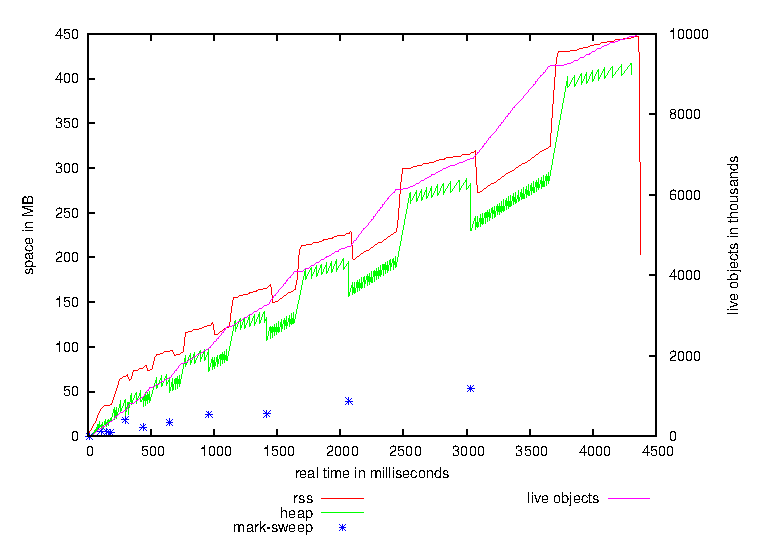
\includegraphics[width=0.5\textwidth]{keep_all_obj_rss_heap_mas_obj_time}
	\caption{Simple mutator which only allocates objects and never deallocates.}
	\label{fig:mutator_keep_all_obj}
\end{figure}

\
Figure \ref{fig:acdc_multi_exec_time} presents the execution time of a mutator which frequently deallocates a static amount of memory. We increase the lifetime of the allocated objects and measure the execution time. The lifetime is the duration since a object is allocated until it is deallocated. The so-called liveness of a object is similar to the lifetime. The x-axis of the figure shows the maximum liveness of the allocated objects and on the y-axis the execution time is displayed. A comparison of Google's V8 with Mozilla's \SM shows significant differences. If we look at the line of V8 we see some big spikes at a liveness of 30, 60, and 90. A reason for these spikes is the communication with the operating system. If the heap size of V8 overruns one of the internal bounds the process requests more memory from the operating system. If the heap size falls below such a bound the process responses memory to the operating system. In our case the heap size is toggling around such bounds. As a result there is a lot more communication with the operation system than usually which has a large impact on the execution time of the mutator.

\
The conclusion of our first mutator measurements is, that we are able to visualize characteristics of a garbage collector. Furthermore, we can show differences between different virtual machines. These mutators represent some corner cases, and if we think of a realistic \JS application there will be a different behavior.

\begin{figure}
	\centering
	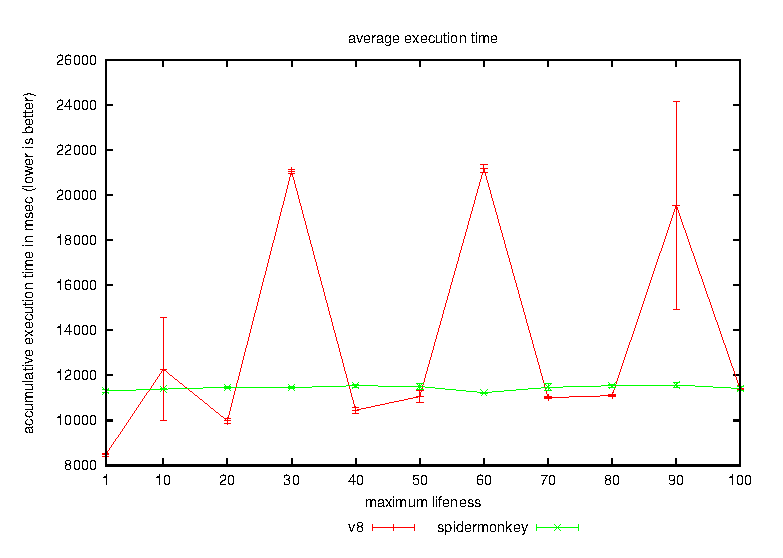
\includegraphics[width=0.5\textwidth]{acdc_multi_exec_time}
	\caption{Execution time: V8 vs. SpiderMonkey}
	\label{fig:acdc_multi_exec_time}
\end{figure}


%%%%%%%%%%%%%%%%%%%%%%%%%%%%%%%%%%%%%%%%%%%%%%%%%%%%%%%%%%%%%%%%%%%%%%%%%%%%%%%%
%%%%%%%%%%%%%%%%%%%%%%%%%%%%%%%%%%%%%%%%%%%%%%%%%%%%%%%%%%%%%%%%%%%%%%%%%%%%%%%%
%%%%%%%%%%%%%%%%%%%%%%%%%%%%%%%%%%%%%%%%%%%%%%%%%%%%%%%%%%%%%%%%%%%%%%%%%%%%%%%%

\subsection{Tools for obtaining a realistic heap model}

Developing a benchmark which is able to simulate a realistic \JS heap requires understanding the heap of real-world applications. As shown by some related work~\cite{JSMeter2009,JSMeter2010,Richards2011} the state-of-the-art benchmarks do not represent realistic heap behavior. In this section we describe our analysis to obtain a realistic heap model.

Our analysis are based on frequent generated snapshots of the \JS heap of a real-world application. The list of analyzed applications and proceeded user interactions is shown in Table \ref{tab:real_world_apps} on page \pageref{tab:real_world_apps}.
Figure \ref{fig:heap_structure_analysis} presents the complete toolchain we used to generate and analyze these snapshots. 

For the simulation of a realistic user interaction on a real-world application we used Selenium \cite{Selenium}. All user interactions we analyze are collected in the so-called \texttt{AutomatedUserInteraction} tool (see Section \ref{sec:automated_user_interaction}). For execution of a interaction we use a custom version of Chromium. We add a mechanism that periodic produces a snapshot of the \JS heap (for details see Section \ref{sec:custom_chromium}). 
The so-called \texttt{HeapSnapshotAnalyzer} analyzes these snapshots. The exact process is explained in Section \ref{sec:heap_snapshot_analyzer}.

\begin{figure}
	\centering
	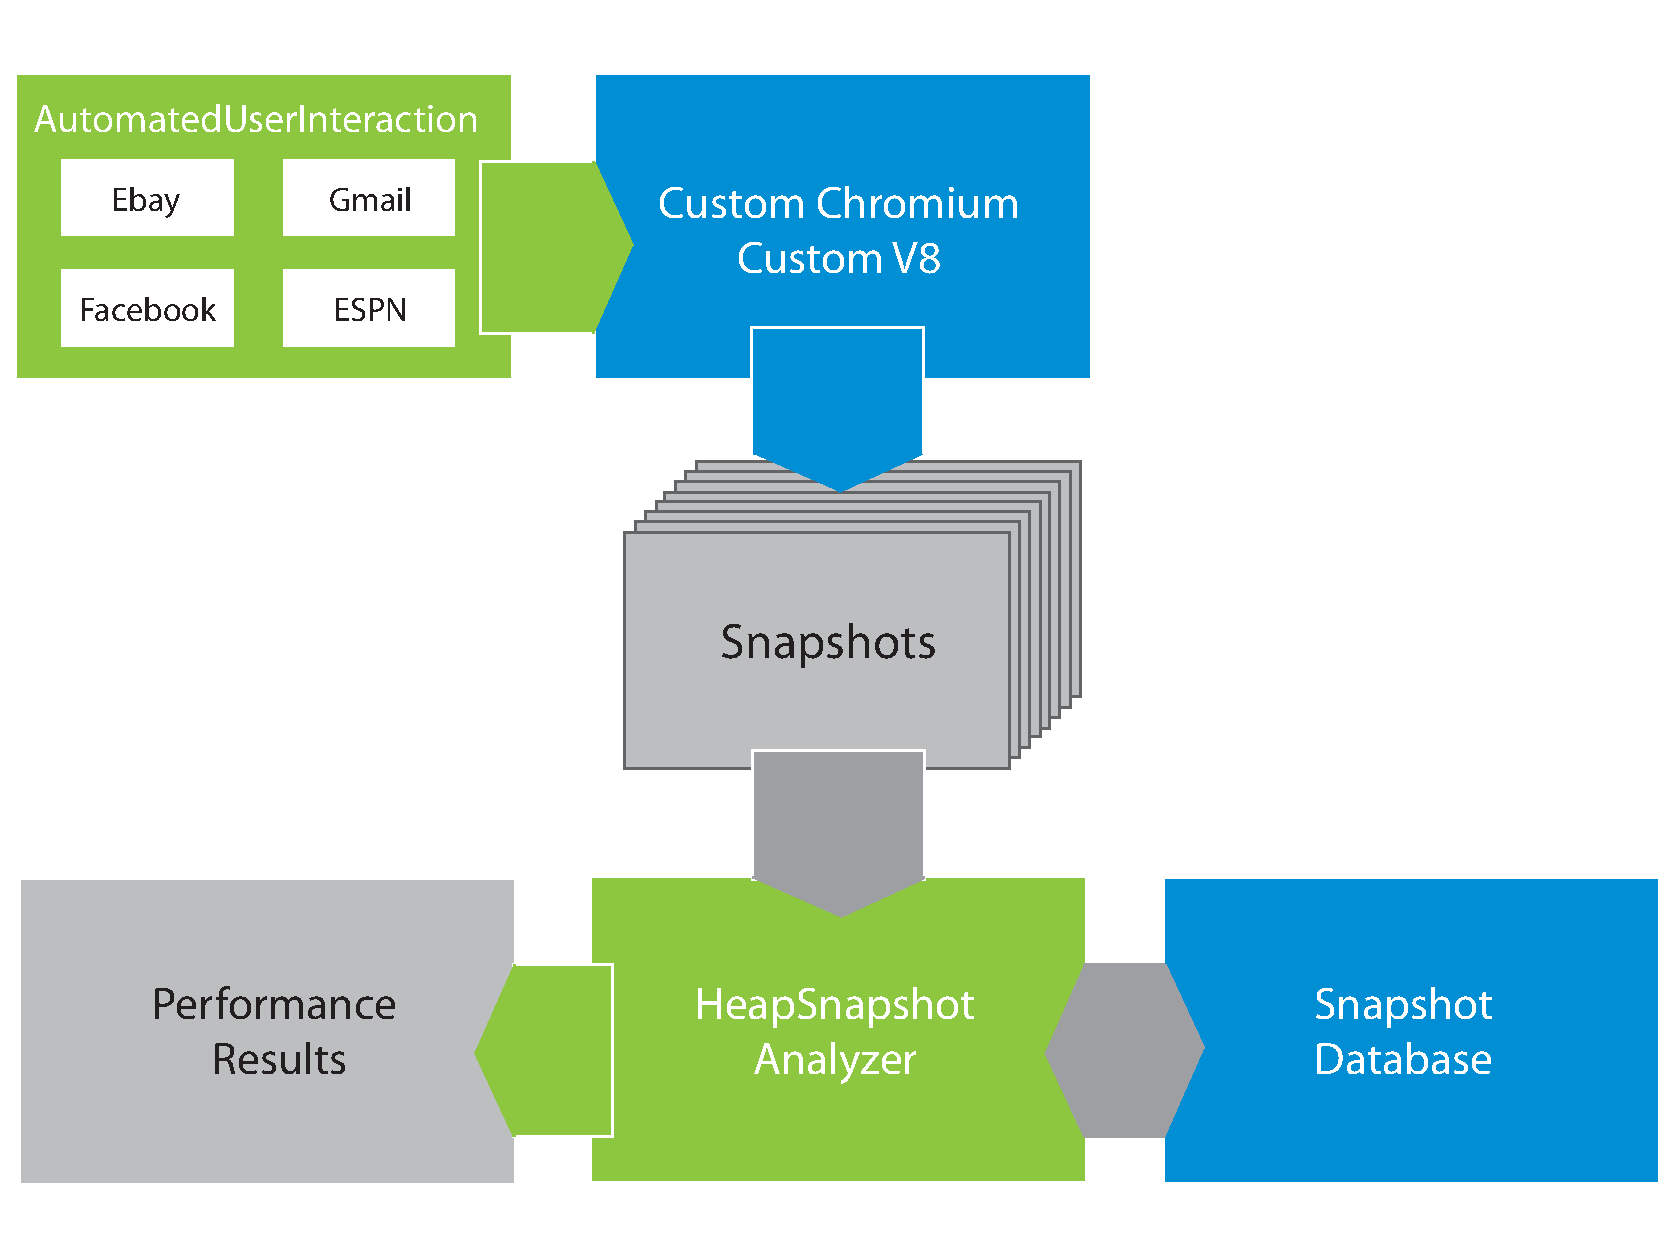
\includegraphics[width=0.5\textwidth]{solution_h}
	\caption{Tool chain for analyzing the JavaScript heap of a real-world web application}
	\label{fig:heap_structure_analysis}
\end{figure}


%%%%%%%%%%%%%%%%%%%%%%%%%%%%%%%%%%%%%%%%%%%%%%%%%%%%%%%%%%%%%%%%%%%%%%%%%%%%%%%%
%%%%%%%%%%%%%%%%%%%%%%%%%%%%%%%%%%%%%%%%%%%%%%%%%%%%%%%%%%%%%%%%%%%%%%%%%%%%%%%%
%%%%%%%%%%%%%%%%%%%%%%%%%%%%%%%%%%%%%%%%%%%%%%%%%%%%%%%%%%%%%%%%%%%%%%%%%%%%%%%%
	
\subsubsection{Tool for automating user interaction} \label{sec:automated_user_interaction}
To simulate a realistic user interaction we decided to automate this process by using Selenium \cite{Selenium}. A benefit of using Selenium is that we are able to repeat a user interaction as often as we want in exact the same way. Selenium also enables the opportunity to use different browsers. This feature allows us to run a user interaction on different browsers or use our own browser binary in a very easy way. For the heap snapshot generation we use our own custom Chromium binary (for details see Section \ref{sec:custom_chromium}). The Table \ref{tab:real_world_apps} shows all these real-world applications and the user interaction we perform. For each kind of web application the user interaction is tailored individually. The collection of all user interactions and a mechanism to switch between different browser binaries is provided by the so-called \texttt{AutomatedUserInteraction} tool.

\begin{table}
	\small
	\centering
	\begin{tabular}{l l}
		\toprule
		\textbf{Site} & \textbf{User interaction} \\ \midrule

		CNN 					& Read start page news, switch to category \textit{Europe}, 			\\ 
		\url{cnn.com} 			& read first article of \textit{Top Europe Stories}. 					\\ \midrule

		The Economist 			& Read start page news, switch to category 								\\ 
		\url{economist.com}		& \textit{Science \& technology}, read first article. 					\\ \midrule

		ESPN 					& Read start page news, switch to \textit{NASCAR}, 		 				\\ 
		\url{espn.com} 			& click on \textit{Results} and read site. 								\\ \midrule

		Hotmail 				& Sign in, check in-box, send email, read an email,						\\ 
		\url{hotmail.com} 		& delete it, and sign out. 												\\ \midrule

		Gmail 					& Sign in, check in-box, send email, read an email, 						\\ 
		\url{www.gmail.com} 	& delete it, and sign out. 												\\ \midrule

		Bing Search 			& Search for \textit{New York} and look at 								\\ 
		\url{bing.com} 			& resulting images and news. 											\\ \midrule

		Google Search 			& Search for \textit{New York} and look at 								\\ 
		\url{google.com}		& resulting images and news. 											\\ \midrule

		Facebook 				& Login and post a message. 											\\ 
		\url{facebook.com} 		&  																		\\ \midrule

		Google+ 				& Login and post a message. 											\\ 
		\url{plus.google.com} 	& 																		\\ \midrule

		Bing Maps 				& Search for directions from \textit{Austin} to \textit{Houston}		\\ 
		\url{maps.bing.com} 	& by car and walk. 														\\ \midrule

		Google Maps				& Search for directions from \textit{Austin} to \textit{Houston}		\\ 
		\url{maps.google.com} 	& by car and walk. 														\\ \midrule

		amazon 					& Search for the book \textit{Quantitative Computer Architecture},		\\ 
		\url{amazon.com} 		& add to shopping cart, look at cart. 									\\ \midrule

		eBay 					& Search for the book \textit{Quantitative Computer Architecture}. 		\\ 
		\url{www.ebay.co.uk} 	& 																		\\ \bottomrule

	\end{tabular}
	\caption{User interactions performed for the heap analysis of real web applications.}
	\label{tab:real_world_apps}
\end{table}

%%%%%%%%%%%%%%%%%%%%%%%%%%%%%%%%%%%%%%%%%%%%%%%%%%%%%%%%%%%%%%%%%%%%%%%%%%%%%%%%
%%%%%%%%%%%%%%%%%%%%%%%%%%%%%%%%%%%%%%%%%%%%%%%%%%%%%%%%%%%%%%%%%%%%%%%%%%%%%%%%
%%%%%%%%%%%%%%%%%%%%%%%%%%%%%%%%%%%%%%%%%%%%%%%%%%%%%%%%%%%%%%%%%%%%%%%%%%%%%%%%

\subsubsection{Custom Chromium} \label{sec:custom_chromium}
Obtaining a realistic \JS heap model requires information about objects and structure of a heap of a real-world \JS application. As explained in \cite{JSMeter2009} modifying the \JS engine of a browser is a good opportunity to get accurate information about the \JS heap. We use Chromium \cite{Chromium} the open source project of Google Chrome \cite{Chrome} to capture information about the \JS heap.

The Google DevTools \cite{DevTools} provide a functionality to generate heap snapshots. The problem is, there is no opportunity to periodic generate such a heap snapshot. We extend the V8 and implement such a mechanism that also stores the generated snapshots at a given directory. This mechanism works by using the Google V8 API function \texttt{TakeHeapSnapshot}. These snapshots contain some meta information, a nodes array, an edges array and a strings array. The nodes array and edges array represent a directed graph, the heap. The strings array is referenced by the nodes and edges array and contains only names. The complete list of properties of a node in the nodes array is shown in Table \ref{tap:heap_snapshot_node_fields} and the properties of the edges are shown in Table \ref{tap:heap_snapshot_edge_fields}. To control the generation of heap snapshots, we extend the V8 with following flags:
\begin{itemize}
	\item \texttt{automatic heap snapshots}
	\item \texttt{heap snapshot interval}
	\item \texttt{heap snapshot prefix} 
\end{itemize}	
The \texttt{automatic heap snapshots} flag enables the generation of snapshots in general, default it is \texttt{false}. To control how frequent snapshots are generated the \texttt{heap snapshot interval} flag is used, default value is 64KB. Every time \texttt{n} KB are allocated a snapshot is taken. The third flag, \texttt{heap snapshot prefix}, is only a prefix of the generated snapshot files, default value is \textit{snapshot}. The produced snapshots are numbered consecutively until the \texttt{automatic heap snapshots} flag is set to \texttt{false} or the mutator terminates. The extension of such files is \textit{.heapsnapshot}. 

%%%%%%%%%%%%%%%%%%%%%%%%%%%%%%%%%%%%%%%%%%%%%%%%%%%%%%%%%%%%%%%%%%%%%%%%%%%%%%%%
%%%%%%%%%%%%%%%%%%%%%%%%%%%%%%%%%%%%%%%%%%%%%%%%%%%%%%%%%%%%%%%%%%%%%%%%%%%%%%%%
%%%%%%%%%%%%%%%%%%%%%%%%%%%%%%%%%%%%%%%%%%%%%%%%%%%%%%%%%%%%%%%%%%%%%%%%%%%%%%%%

\subsubsection{Tool for analyzing heap snapshots} \label{sec:heap_snapshot_analyzer}
The steps before describe how we capture data about a realistic \JS heap. Now we want to explain how we analyze the generated snapshots. 

For each real-world application, listed in Table \ref{tab:real_world_apps}, we use a sample rate of 4KB, i.e., a snapshot is created whenever 4KB of new objects are allocated by the application. The number of generated snapshots depends on the amount of memory which is allocated by a real-world application and the runtime of a user interaction. When a heap snapshot is taken the garbage collector is automatically called. As a result a snapshot only contains live objects. 

However, we use a PostgreSQL \cite{PSQL} database, version 9.3, to analyze the snapshots. To handle the preparation of a snapshot for the database as well as the analysis we develop a tool. This tool is a Java application that we call \texttt{HeapSnapshotAnalyzer}. For a realistic heap model, we are interested in the distribution of object types, sizes and lifetimes, the number of out-going edges, and the distance from a GC root to a object. A heap snapshot represents all live objects of the \JS heap and each object has a type. The complete list of object types is shown by Table \ref{tap:heap_snapshot_node_types}. An object also has a size, which represents the amount of byte the object needs on the heap. The number of outgoing edges represents the number of references an object holds. A snapshot contains special nodes of type synthetic which represent GC roots. These nodes has are used to compute the root distance. The root distance represents the minimum number of edges to reach a node from a GC root. How we compute these properties is described in Section \ref{sec:analysis_mutator}.
	%-------------------------------------------------------------------
% bachelor thesis
% create by: Mario Preishuber
% create date: 2014, Jan 01.
%-------------------------------------------------------------------

\section{Mutator Heap Analysis} \label{sec:analysis_mutator}

In this section we describe how to some interesting heap properties and present our analysis results of the mutator heap. For our analysis we only care about object types which can be allocated by a mutator. These object types are arrays, strings, user-defined objects, code, closures, regular expressions (regexp), and numbers. We analyzed the distribution of object types, sizes and lifetimes, the number of outgoing edges, and the distance from the GC roots to the objects. 
The type information is part of a heap snapshot. The distribution of object types is computed over all workloads, i.e., all snapshots of all real-world application. Figure \ref{fig:obj_alloc_dist} presents the distribution of object types as a histogram. A heap snapshot contains not only objects with a type presented in the histogram. There are several V8 specific types like hidden classes which describe a internal representation of object properties, and GC roots have the type synthetic. We do not care about the V8 specific types, to be platform independent. Our analysis show that the most objects are of type array, string, or user-defined object. The dominance of arrays differs from the results in \cite{JSMeter2009}. A reason for this behavior is if it is necessary to a copy an array because it grows too much, we treat the new array logically as a new heap object. This behavior results in an increasing number of objects and the average lifetime decreases. 
\begin{figure}
	\centering
	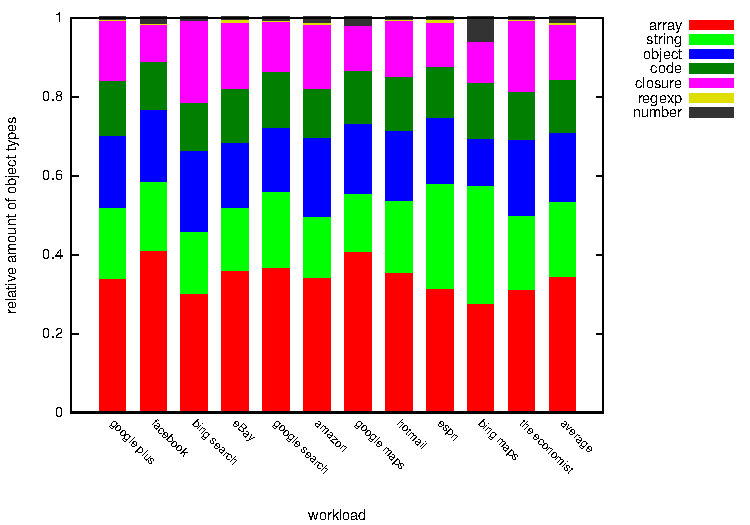
\includegraphics[width=0.5\textwidth]{obj_alloc_dist}
	\caption{Histogram of the object type distribution for all workloads, confirms \cite{JSMeter2009}.}
	\label{fig:obj_alloc_dist}
\end{figure}

Figure \ref{fig:obj_selfsize_dist} shows the object size distribution for each type. The x-axis displays the object size in byte and the y-axis shows the relative amount of objects living shorter than x. Each object on the \JS heap is identified by a unique V8 internal id which is a property of a heap snapshot. The size of a object is also a property of a snapshot. This allows us to count objects of the same size of all snapshots of all workloads. As the figure shows depends the object size distribution on the type of the objects. There are a few large object and a lot of small objects. This behavior is similar to the allocation behavior of C programs which is shown in \cite{Aigner2013}. The figure also shows that there are object types with a fix size, e.g., numbers with a size of 12 byte.
\begin{figure}
	\centering
	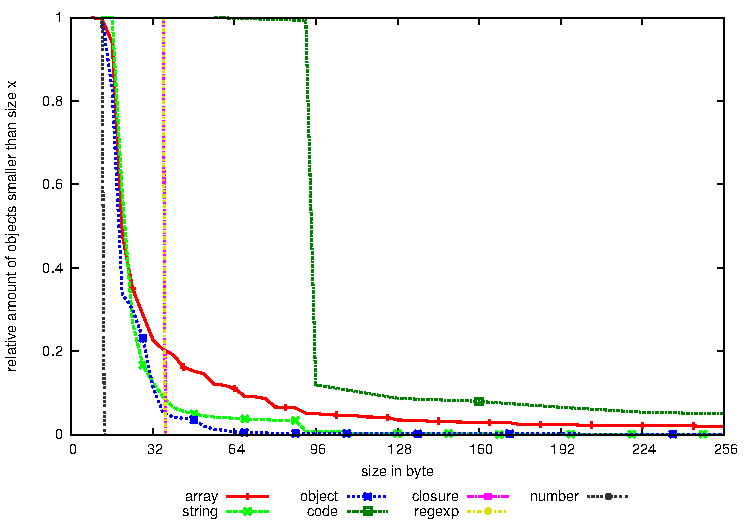
\includegraphics[width=0.5\textwidth]{obj_selfsize_dist}
	\caption{Size distribution of real web applications, confirms \cite{JSMeter2009}.}
	\label{fig:obj_selfsize_dist}
\end{figure}

As explained above it is possible to identify an object by an unique id which never changes. This fact allows us to compute the lifetime of an object. Figure \ref{fig:obj_lifetime_dist} illustrates the distribution of the lifetime of all snapshots of all workloads separated by the object type. The lifetime is measured in allocated bytes which are allocated during a object is live. As a result of the sampling rate of the snapshot generation which is 4 KB, the minimum lifetime of a object is also 4 KB. These amount of allocated byte is displayed on the x-axis and on the y-axis is the relative amount of objects living shorter than x presented. The figure shows that the lifetime of arrays is significant smaller the lifetime of strings. What results of the fact, if a array has to be copied, because of growing too much, a logically new array is created. This approach influences the liveness of arrays, but from the garbage collector perspective this way of counting is okay, because the old array also has to be deallocated.
\begin{figure}
	\centering
	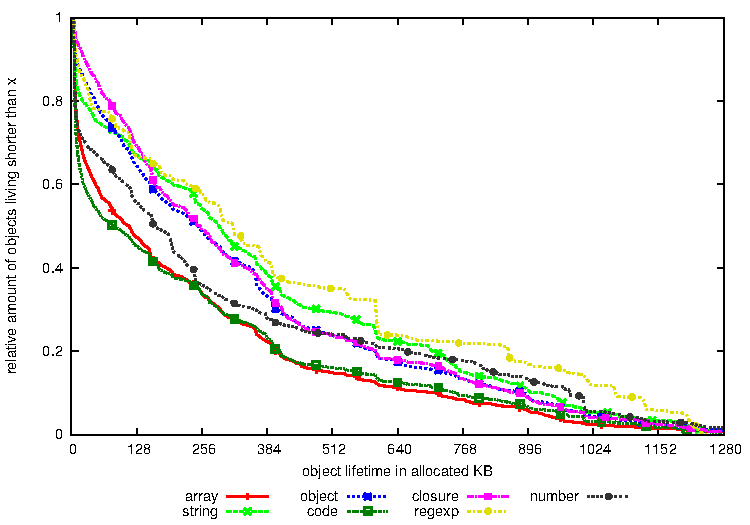
\includegraphics[width=0.5\textwidth]{obj_lifetime_dist}
	\caption{Lifetime distribution of real web applications, confirms \cite{JSMeter2009}.}
	\label{fig:obj_lifetime_dist}
\end{figure}

An important property of a heap structure is the depth of a heap graph. So we computed the minimum distance of a node to it's GC root. A heap snapshot contains special nodes which represent GC roots, these nodes are of the type synthetic. We use a recursive depth-first search algorithm and compute the root distance for each node of all snapshots of all workloads and separated again by type. The x-axis of Figure \ref{fig:obj_rootdist_dist} shows the minimum root distance and the y-axis presents the relative amount of objects with a root distance smaller than x. This figure shows that the most objects have a small root distance.
\begin{figure}
	\centering
	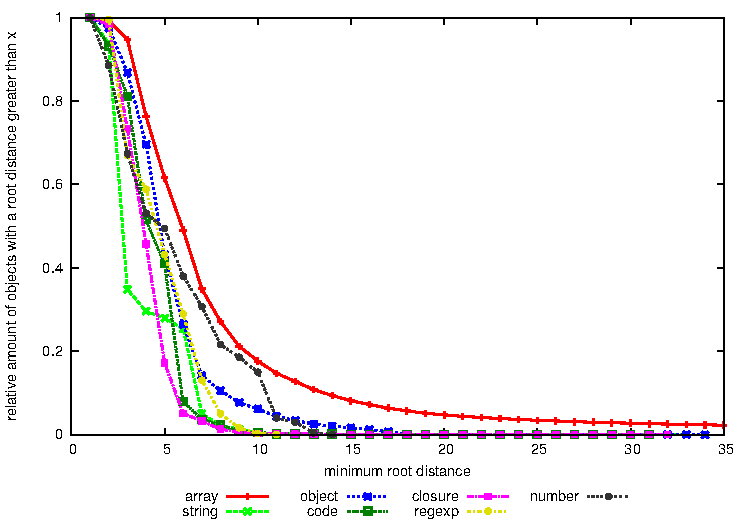
\includegraphics[width=0.5\textwidth]{obj_rootdist_dist}
	\caption{GC root distance distribution of real web applications, confirms \cite{JSMeter2009}.}
	\label{fig:obj_rootdist_dist}
\end{figure}

Another interesting property by talking about the structure of a heap is the number of outgoing edges of a node. The number of outgoing edges, the so-called out-degree, results of the fact that the snapshots represent a directed graph. So this information is provided by the heap snapshots. Figure \ref{fig:obj_outdeg_dist} shows the distribution of the out-degree separated by the object type. The out-degree is computed for each node of each snapshot of all workloads. The x-axis of the figure presents the out-degree and on the y-axis is the relative amount of objects with an out-degree smaller than x displayed. Arrays have a low out-degree what indicates that most arrays contain primitive types. 
\begin{figure}
	\centering
	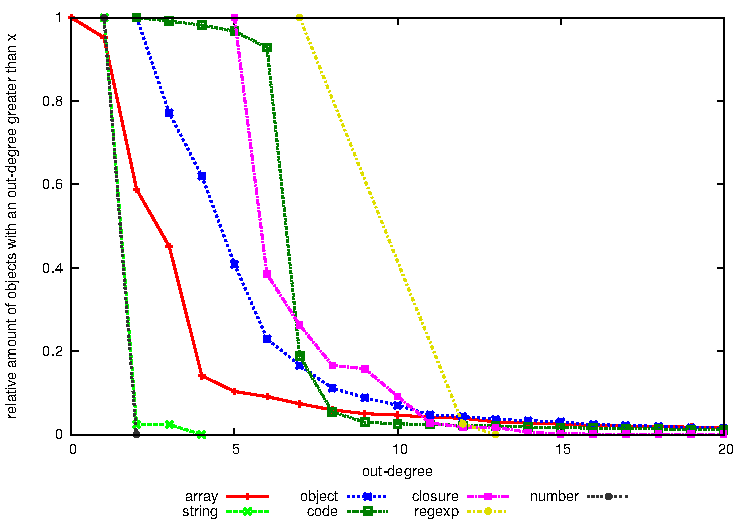
\includegraphics[width=0.5\textwidth]{obj_outdeg_dist}
	\caption{Out-degree distribution of real web applications, confirms \cite{JSMeter2009}.}
	\label{fig:obj_outdeg_dist}
\end{figure}

If we talk about the out going edges of a node we want also to know how the number of in-going edges looks like. The number of in-going edges, the so-called in-degree, is not an explicit property of a snapshot, i.e., it requires some computations. In other words the in-degree represents the number of parents a node has and this is the way how it is computed. Before inserting a snapshot into the database some preparations are required and during these preparations the number of parents of a node is counted. Figure \ref{fig:obj_indeg_dist} shows the distribution of the in-degree over all nodes of all snapshots of all workloads separated by type. On the x-axis is the in-degree displayed and on the y-axis is the relative amount of objects with an in-degree smaller than x is shown. The figure presents a quite different behavior than Figure \ref{fig:obj_outdeg_dist} which shows the out-degree distribution. The behavior of the different types is more similar that it is for the out-degree. As expected have strings a higher in-degree, because often are strings allocated once and reused.
\begin{figure}
	\centering
	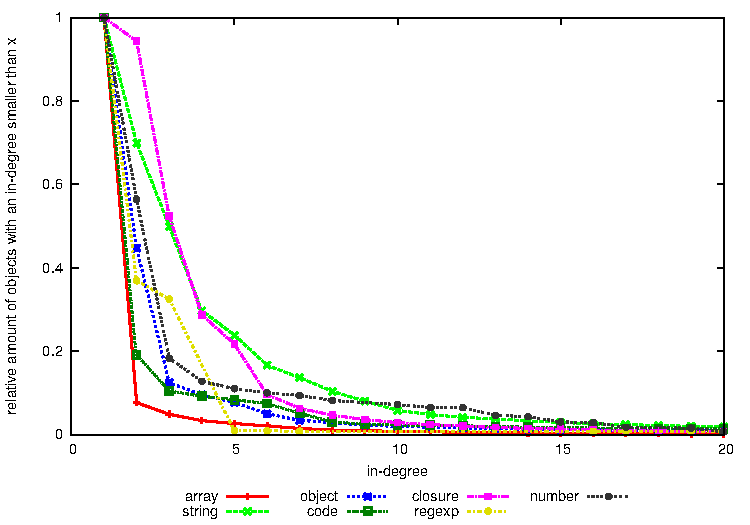
\includegraphics[width=0.5\textwidth]{obj_indeg_dist}
	\caption{In-degree distribution of real web applications, confirms \cite{JSMeter2009}.}
	\label{fig:obj_indeg_dist}
\end{figure}

To complete our analysis of the heap structure we have a look at strongly connected components. We compute the strongly connected components with the Trajan's algorithm \cite{Trajan}. We are interested in the size of a strongly connected component, i.e., the number of edges which the components contains. What we also want to know is the number of strongly connected components of a heap graph. One snapshot represents the current heap, since a heap is a directed graph we analyzed each snapshot separate. The Table \ref{tab:scc_stats} shows our analysis results, the values are the average values of all snapshots of all workloads. If we compare the average and the median of the quantity we recognize a significant difference. This comparison shows there are some extreme values, which is also illustrated by the maximum, but the most heaps contain less then 50 strongly connected components. The size of these strongly connected components presents a similar result. There are a lot of small strongly connected components and a few large.
\begin{table}
	\small
	\centering
	\begin{tabular}{l r r}
		\toprule
		\textbf{strongly connected components} & \textbf{size} & \textbf{quantity} \\ \midrule
		minimum							&	0.286		&	0.782			\\ 
		maximum							&	53,729.857	&	285.916			\\ 
		average							&	5,316.409	&	11.177			\\ 
		quantile 25						&	2,304.786	&	3.107			\\ 
		quantile 50						&	3,082.429	&	6.329			\\ 
		quantile 75						&	3,629.714	&	14.655			\\ 
		quantile 90						&	12,199.429	&	36.211			\\ 
		quantile 95						&	25,979.000	&	49.448			\\ \bottomrule
	\end{tabular}
	\caption{Summary of the measurements of strongly connected components.}
	\label{tab:scc_stats}
\end{table}
	%-------------------------------------------------------------------
% bachelor thesis
% create by: Mario Preishuber
% create date: 2014, Jan 01.
%-------------------------------------------------------------------

\section{System Heap Analysis}  \label{sec:analysis_system}

In this section we present our analysis results of the system heap. For our analysis we only care about objects of type hidden, native, or synthetic. Objects of type hidden represent hidden classes. These objects are generated by Google's V8 and represent the properties of a object. GC roots has the type synthetic and objects of type native represent other objects, i.e., DOM roots. We analyze the same properties as described in Section \ref{sec:analysis_mutator} in the same way.

The result of the object type distribution of the system types show that about 99\% of these objects are of type hidden, this holds for all workloads. There are extreme few objects of the types synthetic and native. One reasons is that objects of type synthetic represent GC roots and it is plausible that there are not much such objects. Nevertheless, we care about them, because of completeness.

Figure \ref{fig:obj_sys_selfsize_dist} illustrates the size distribution of the system object types of all snapshots over all workloads. The size of native and synthetic objects is always zero in a heap snapshot. This is a special behavior and represents not the real size of these objects. Nevertheless, is Figure \ref{fig:obj_sys_selfsize_dist} interesting because is shows the size distribution of hidden classes. On the x-axis of the figure the size in byte and on the y-axis the relative amount of objects smaller than size x. We see that there are only few objects of type hidden with a size larger than 64 byte. It seems that the size of 64 byte is some kind of bound, because there is a hard back. 

\begin{figure}
	\centering
	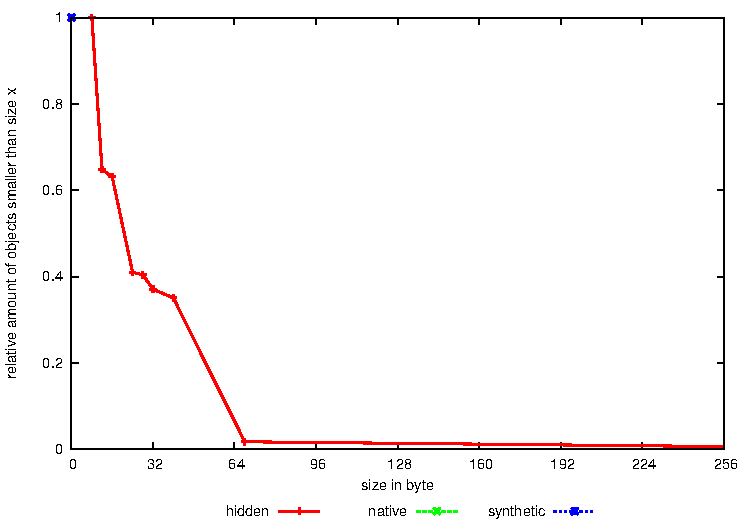
\includegraphics[width=0.5\textwidth]{obj_sys_selfsize_dist}
	\caption{Size distribution of real web applications.}
	\label{fig:obj_sys_selfsize_dist}
\end{figure}

In Figure \ref{fig:obj_sys_lieftiem_dist} we present the lifetime distribution over all snapshots of all workloads separated by the object type. The x-axis shows the object lifetime in allocated KB. We decided to use this metric to get rid of the lifetime in snapshots representation. The sample rate of the snapshot generation is 4KB of allocated memory and this leads to an minimum lifetime of 4KB. The lifetime of hidden classes shows a similar behavior than the lifetime of mutator objects of type user-defined object as explained in Section \ref{sec:analysis_mutator}, especially Figure \ref{fig:obj_lifetime_dist} on page \pageref{fig:obj_lifetime_dist} illustrates this behavior.

\begin{figure}
	\centering
	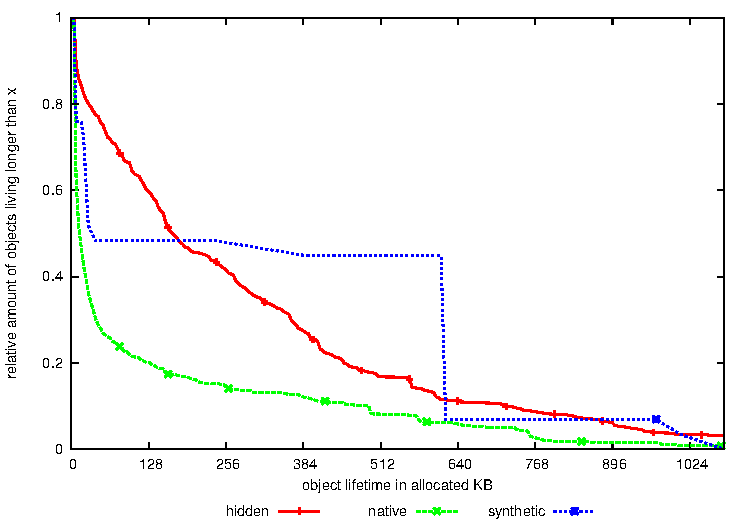
\includegraphics[width=0.5\textwidth]{obj_sys_lifetime_dist}
	\caption{Lifetime distribution of real web applications.}
	\label{fig:obj_sys_lieftiem_dist}
\end{figure}

The root distance of nodes in a graph is an interesting parameter of the graph characteristic. If we look at the root distance of system objects we face some special cases, because objects of type synthetic represent GC roots that are used to compute the root distance. It is possible that an object of type synthetic also has an root object. So the root distance of synthetic objects is always zero or one. Objects of type native show a similar behavior because these are also used to represent DOM roots. Nevertheless, the behavior of objects of type hidden provides interesting information. Figure \ref{fig:obj_sys_rootdist_dist} illustrates the root distance distribution of system objects. The x-axis of the figure shows the minimum root distance and the y-axis the relative amount of objects with a root distance smaller than x. We conclude that hidden classes have a small root distance and that there are only few objects with a higher root distance.

\begin{figure}
	\centering
	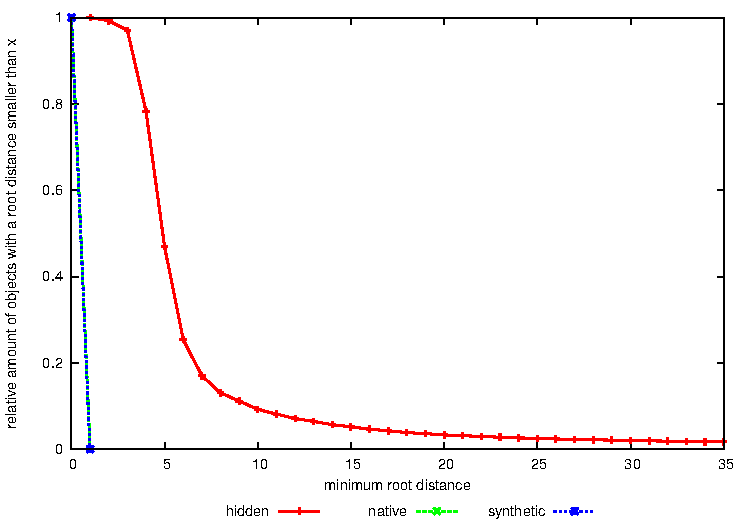
\includegraphics[width=0.5\textwidth]{obj_sys_rootdist_dist}
	\caption{Root distance distribution of real web applications.}
	\label{fig:obj_sys_rootdist_dist}
\end{figure}

The Figure \ref{fig:obj_sys_outdeg_dist} presents the distribution of outgoing
edges of a node, the so-called out-degree. This illustration shows the results
computed over all snapshots of all workloads. In this figure we see that
objects of type hidden have a out-degree of less than ten. If we have a look at
the native line, we recognize that this kind of objects have a significantly
higher out-degree than objects of type hidden. Especially objects of type
synthetic have a extreme high out-degree, because they represent the GC roots
and we conclude that the heap tree is very breadth.

\begin{figure}
	\centering
	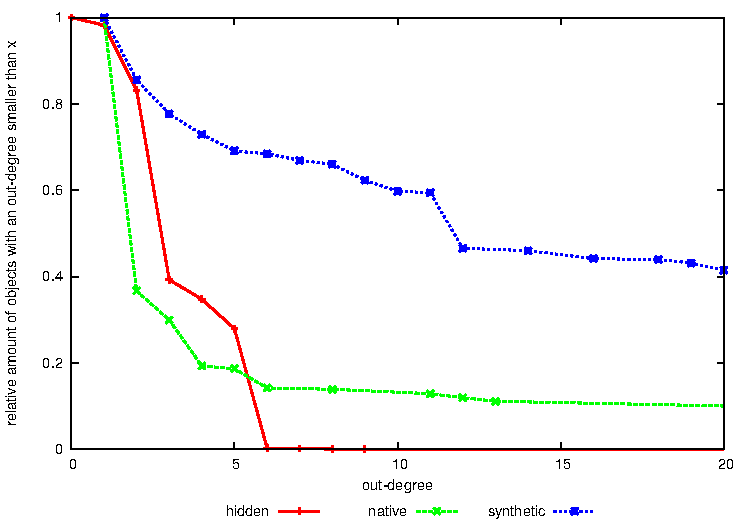
\includegraphics[width=0.5\textwidth]{obj_sys_outdeg_dist}
	\caption{Out-degree distribution of real web applications.}
	\label{fig:obj_sys_outdeg_dist}
\end{figure}

% \begin{figure}
% 	\centering
% 	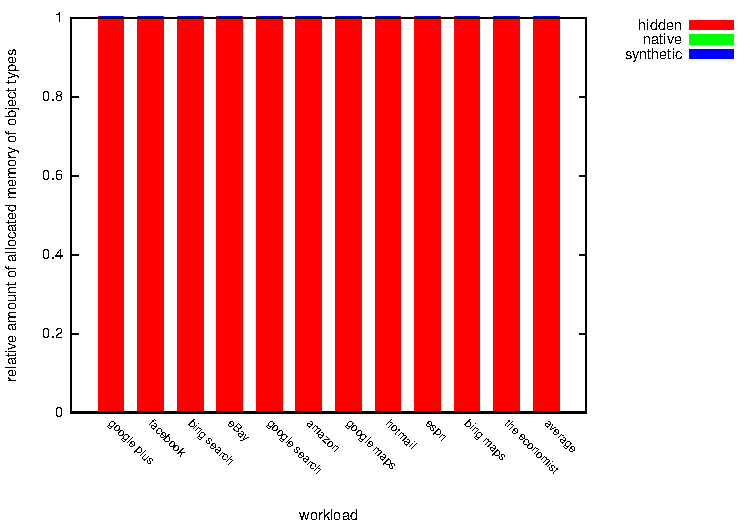
\includegraphics[width=0.5\textwidth]{obj_sys_byte_dist}
% 	\caption{Histogram of the object type distribution for all workloads.}
% 	\label{fig:obj_sys_byte_dist}
% \end{figure}
% 
% \begin{figure}
% 	\centering
% 	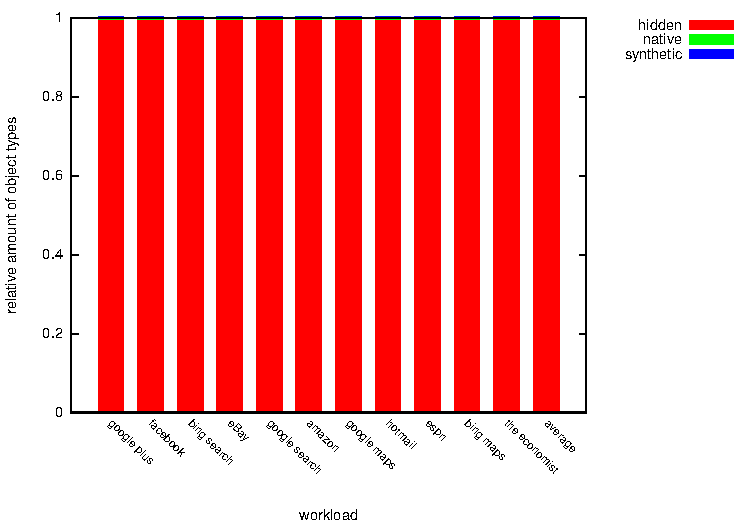
\includegraphics[width=0.5\textwidth]{obj_sys_alloc_dist}
% 	\caption{Histogram of the object type distribution for all workloads.}
% 	\label{fig:obj_sys_alloc_dist}
% \end{figure}

	%-------------------------------------------------------------------
% bachelor thesis
% create by: Mario Preishuber
% create date: 2014, Jan 01.
%-------------------------------------------------------------------

\section{System vs. Mutator} \label{sec:analysis_sys_vs_mut}

In the previous sections we described our analysis results separated in system objects and mutator objects. We presented the differences and similarities distinguished by the type of the objects. In this section we compare system and mutator objects and do not care about the type of the objects. As explained in the section \ref{sec:analysis_mutator} are objects of type array, string, user-defined object, code, closure, regular expression (regexp), or number mutator objects. Objects of type hidden, native, or synthetic are system objects as described in section \ref{sec:analysis_system}. This analysis illustrate the overhead produced by Google's V8. 

Figure \ref{fig:obj_sysmut_alloc_dist} shows a histogram of the object distribution for all workloads. On the x-axis the workloads are listed and on the y-axis the relative amount of objects is displayed. This Figure shows that there are about 25\% of the allocated objects are system objects. As explained in section \ref{sec:analysis_system} most of these objects are of type hidden. 
\begin{figure}
	\centering
	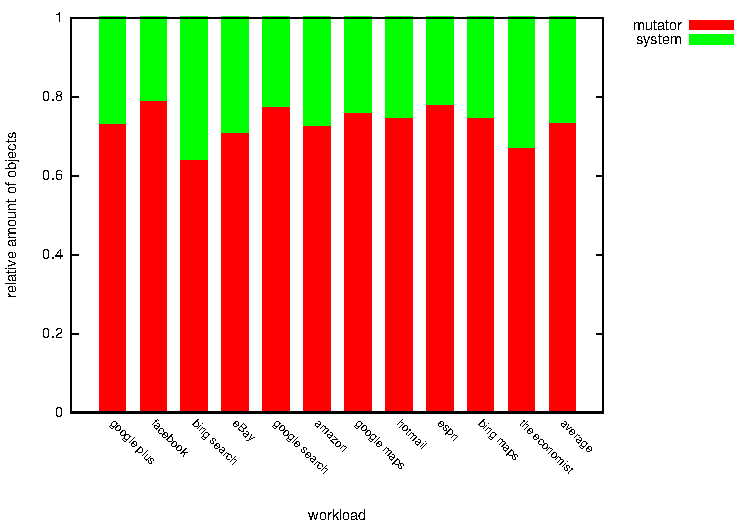
\includegraphics[width=0.5\textwidth]{obj_sysmut_alloc_dist}
	\caption{Histogram of the object distribution for all workloads.}
	\label{fig:obj_sysmut_alloc_dist}
\end{figure}

The distribution of the out-degree is presented by Figure \ref{fig:obj_sysmut_outdeg_dist}. On the x-axis is the out-degree shown and on the y-axis the relative amount of objects with an out-degree smaller than x is presented. This Figure shows a quite different behavior of system and mutator objects. The only similarity is that there are few objects with an out-degree higher than six. More detailed, there are less than 1\% of system and less than 10\% of mutator objects with a higher out-degree than six. It is also interesting that the out-degree of mutator objects is significantly smaller as the out-degree of system objects.
\begin{figure}
	\centering
	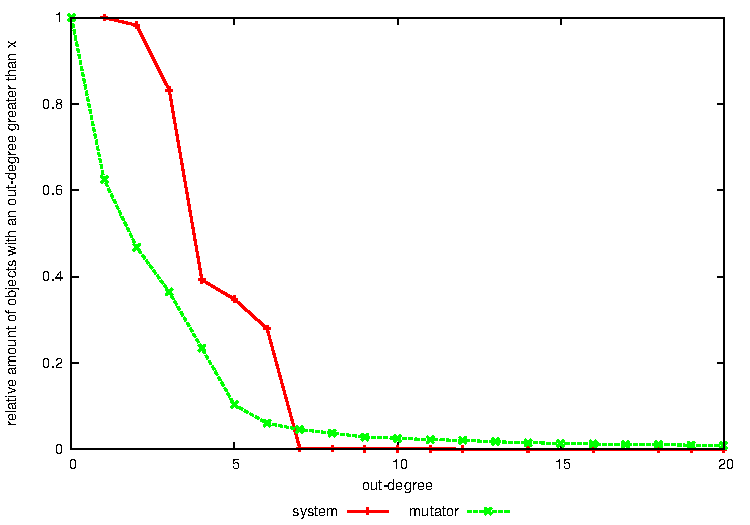
\includegraphics[width=0.5\textwidth]{obj_sysmut_outdeg_dist}
	\caption{Out-degree distribution of real web applications.}
	\label{fig:obj_sysmut_outdeg_dist}
\end{figure}

The lifetime distribution, illustrated by Figure \ref{fig:obj_sysmut_lieftiem_dist}, presents a similar behavior of system and mutator objects. A reason for this is the dependency of hidden classes and user-define objects and again the fact that most of the system objects are of the type hidden. On the x-axis of the Figure the object lifetime in allocated KB is shown and on the y-axis the relative amount of objects living shorter than x is displayed. 
\begin{figure}
	\centering
	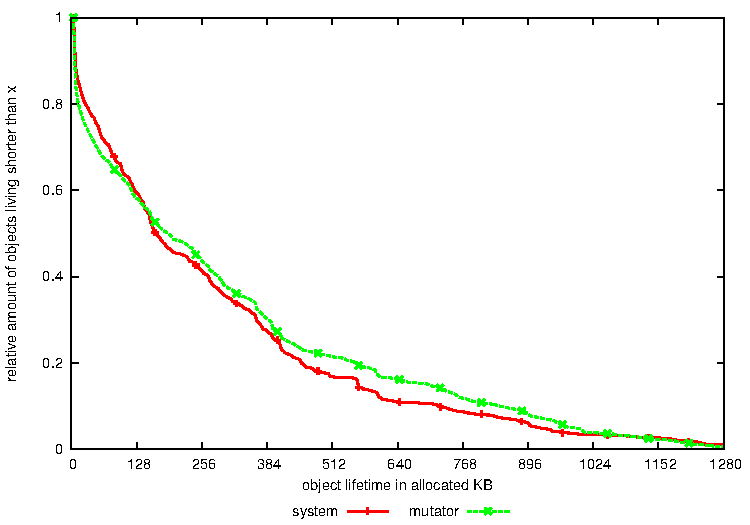
\includegraphics[width=0.5\textwidth]{obj_sysmut_lifetime_dist}
	\caption{Lifetime distribution of real web applications.}
	\label{fig:obj_sysmut_lieftiem_dist}
\end{figure}

Figure \ref{fig:obj_sysmut_rootdist_dist} presents the distribution of the root distance of all snapshots of all workloads separated in system and mutator objects. On the x-axis the minimum root distance is shown and on the y-axis the relative amount of objects with a root distance smaller than x is shown. The behavior of the system and mutator objects is extremely similar. We conclude that there might be a dependency of the position of system objects and the position of mutator objects in the heap graph. A reason could be that a user-defined objects has a reference the hidden class which represents the properties of a object.  
\begin{figure}
	\centering
	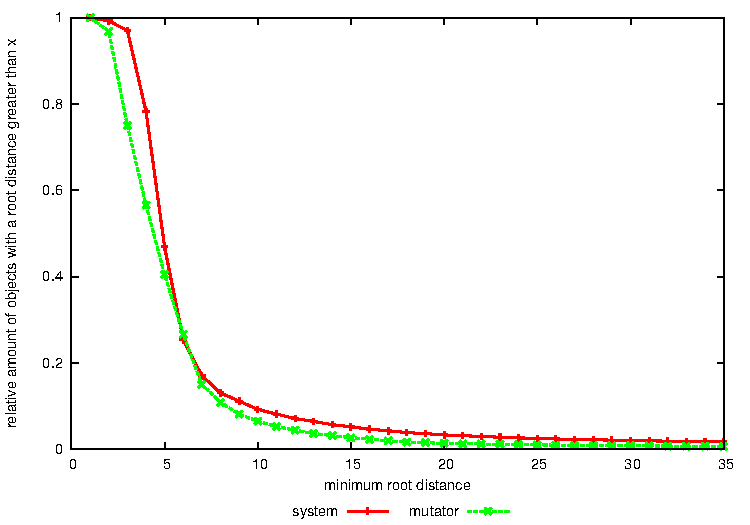
\includegraphics[width=0.5\textwidth]{obj_sysmut_rootdist_dist}
	\caption{Root distance distribution of real web applications.}
	\label{fig:obj_sysmut_rootdist_dist}
\end{figure}

If we compare the size distribution of system and mutator objects we recognize that system objects are significantly bigger. This behavior is illustrated by Figure \ref{fig:obj_sysmut_selfsize_dist}, which shows on the x-axis the size in byte and on the y-axis relative amount of objects smaller than size.
\begin{figure}
	\centering
	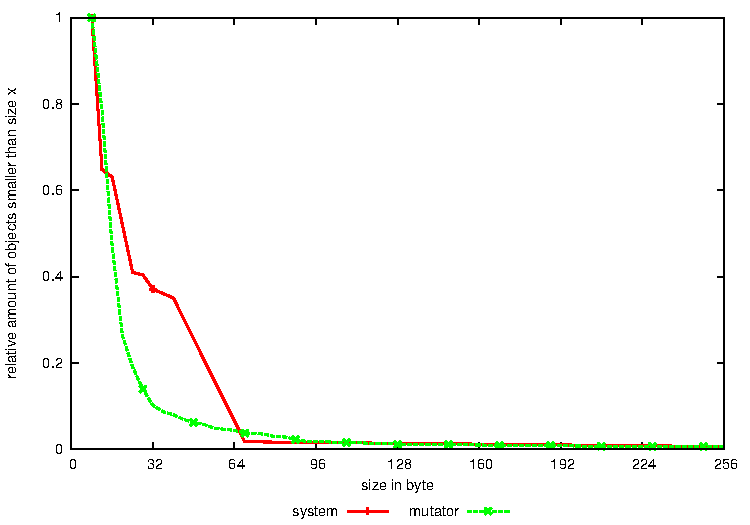
\includegraphics[width=0.5\textwidth]{obj_sysmut_selfsize_dist}
	\caption{Size distribution of real web applications.}
	\label{fig:obj_sysmut_selfsize_dist}
\end{figure}
	%-------------------------------------------------------------------
% bachelor thesis - presentation
%
% topic: ACDC4JS - How to analyze a JavaScript garbage collector
%
% create by: Mario Preishuber
% create date: 2014, Jan 01.
%-------------------------------------------------------------------

\section{Conclusion}
\begin{frame}
	\frametitle{Conclusion}
	Done so far:
	\begin{itemize}
		\item Analyzed garbage collector behavior
		\item Analyzed real web application heap behavior
	\end{itemize}
	To do:
	\begin{itemize}
		\item Complete the implementation of the mutator
	\end{itemize}
\end{frame}
	
	\appendix
	\section{Appendix}

This section presents some additional tables about the generated heap snapshots.

\begin{table}[!htbp]
	\centering
	\begin{tabular}{|l||l|}
		\hline
		\textbf{Name}	&	\textbf{Description}				\\ \hline \hline
		number of nodes & Each snapshot contains a field 
						  called \texttt{node\_count}.  			\\
						& The \texttt{node\_count} field is equal 
						  with \texttt{number of nodes} and			\\
						& shows how many nodes the heap currently 
						  contains. The \texttt{nodes\_count} 		\\
						& field is also an property of the table
						  \texttt{snapshots} and exists once		\\
						& per snapshot.								\\ \hline
		number of edges	& This is the same as \texttt{number of nodes} 
						  only for edges. Each snapshot 			\\
						& contains a field \texttt{edge\_count}. 
						  The \texttt{edge\_count} field is 		\\
						& equal with number of edges and shows how 
						  many edges the heap currently 			\\
						& contains. The \texttt{edge\_count} field 
						  is also an property of the table 			\\
						& \texttt{snapshots} and exists once per 
						  snapshot.									\\ \hline
		number of leafs	& The \texttt{number of leaves} is computed 
						  as followed: scan all nodes of a 			\\
						& snapshot and count those without children. 
						  Each node has a property called 			\\
						& \texttt{edge\_count} this value is 
						  different from the \texttt{edge\_count} 	\\
						& of a snapshot, only the name is the same. 
						  A node has no children if the 			\\
						& \texttt{edge\_count} is zero, because the
						  \texttt{edge\_count} field 				\\
						& contains the number of leaving edges. The
						  \texttt{edge\_count} field it 			\\
						& an property of the \texttt{nodes} table.	\\ \hline
		outdegree		& As explained before each node has a 
						  property \texttt{edge\_count} which 		\\
						& shows the number of leaving edges. 
						  The number of leaving edges is the same 	\\
						& as the outdegree of a node, so it follows 
						  that \texttt{edge\_count} is also 		\\
						& equal with the outdegree of a node. By 
						  using some aggregations of SQL it is 		\\
						& easy to compute the maximum, minimum and 
						  average number of leaving edges. 			\\
						& The \texttt{edge\_count} field it an 
						  property of the \texttt{nodes} table.		\\ \hline
		indegree		& The \texttt{indgeree} of a node is 
						  computed before inserting the data into	\\
						& the database. For each node in the 
						  snapshot is counted how many other nodes	\\
						& have a reference to this.					\\ \hline
		selfsize		& The \texttt{selfsize} is a property of a 
						  node in the snapshot and is 				\\
						& computed by the V8 snapshotting mechanism. 
						   It shows the size of a node in			\\
						& byte.										\\ \hline 
		rootdistance	& The \texttt{rootdistance} is an property 
						  of the \texttt{node} table and is 		\\
						& computed for each node before it is 
						  inserted in the database. 				\\
						& The rootdistance is the shortest path from 
						   any root to a node.						\\ \hline
		strongly		& To find strongly connected components in 
						  the heap graph the Tarjan's 				\\ 
		connected		& strongly connected components
			 			  algorithm\cite{Trajan} is used.			\\
		components		&											\\ \hline
	\end{tabular}
	\caption{Heap snapshot metrics}
	\label{tap:heap_snapshot_metrics}
\end{table}

\begin{table}[!htbp]
	\centering
	\begin{tabular}{|l||l|}
		\hline
		\textbf{Field name}	& \textbf{Description} 				\\ \hline \hline
		type & See Table \ref{tap:heap_snapshot_node_types}			\\ \hline
		name & A string which names the object. If the object is	\\
			 & an mutator variable this name is the same as in 		\\
			 & the mutator (reference to strings array)				\\ \hline	
		id	 & A unique id given by the virtual machine (V8)		\\ \hline
		selfsize  & This is the size of the object in byte. 		\\ \hline
		edgecount &	Number of reference which leaves the object.	\\ \hline	
	\end{tabular}
	\caption{Heap snapshot node fields}
	\label{tap:heap_snapshot_node_fields}
\end{table}
		
\begin{table}[!htbp]
	\centering
	\begin{tabular}{|l||l|}
		\hline
		\textbf{Field name}	&	\textbf{Description}			\\ \hline \hline
		type & See Table \ref{tap:heap_snapshot_edge_types}		\\ \hline
		name\_or\_index & A string which names the edge. 
							(reference to strings array)		\\	\hline
		to\_node		& It is the pointer to the child node. 
							(reference to nodes array)			\\	\hline 
	\end{tabular}
	\caption{Heap snapshot edge fields}
	\label{tap:heap_snapshot_edge_fields}
\end{table}
		
\begin{table}[!h]
	\centering
	\begin{tabular}{|l||l|}
		\hline
		\textbf{Name} & \textbf{Description} 					\\ \hline \hline
		context  & A variable from a function context			\\ \hline
		element  & An element of an array 						\\ \hline
		property & A named object property						\\ \hline
		internal &	A link that can't be accessed from JS, thus,\\
				 & its name isn't a real property name 
				  	(e.g. parts of a ConsString)				\\ \hline
		hidden	  & A link that is needed for proper sizes 
		 			calculation, 								\\
				  & but may be hidden from user					\\ \hline
		shortcut  & A link that must not be followed during	
					sizes calculation							\\ \hline
		weak 	  &	A weak reference (ignored by the GC)		\\ \hline
	\end{tabular}
	\caption{Heap snapshot edge types}
	\label{tap:heap_snapshot_edge_types}
\end{table}
		
\begin{table}[!htbp]
	\centering
	\begin{tabular}{|l||l|}
		\hline
		\textbf{Name} & \textbf{Description} 					\\ \hline \hline
		hidden & Hidden node, may be filtered when shown to user\\ \hline
		array  & An array of elements							\\ \hline
		string & A string										\\ \hline
		object & A JS object (except for arrays and strings)	\\ \hline
		code   & Compiled code									\\ \hline
		closure & Function closure								\\ \hline
		regexp & A regular expression							\\ \hline
		number & Number stored in the heap						\\ \hline
		native & Native object 									\\ \hline
		synthetic & Synthetic object, usually used for grouping 
					snapshot items together						\\ \hline
		concatenated string & Concatenated string 
							(a pair of pointers to strings)		\\ \hline
		sliced string & Sliced string 
						(a fragment of another string)			\\ \hline
	\end{tabular}
	\caption{Heap snapshot node types}
	\label{tap:heap_snapshot_node_types}
\end{table}
	
	\bibliography{bac_strings,thesis}
	
\end{document}